


\begin{figure}[h!]
\center{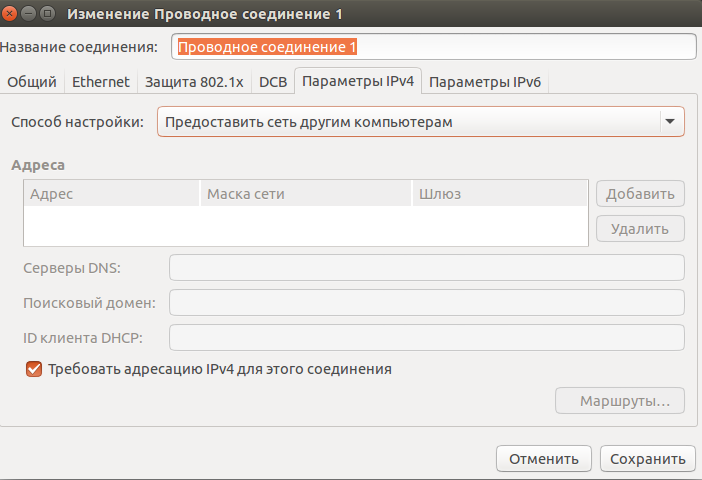
\includegraphics[width=0.6\linewidth]{network_1}}
\caption{ Параметры IPv4 для проводного соединения }
\label{network_1:network_1}
\end{figure}


\begin{figure}[h!]
\center{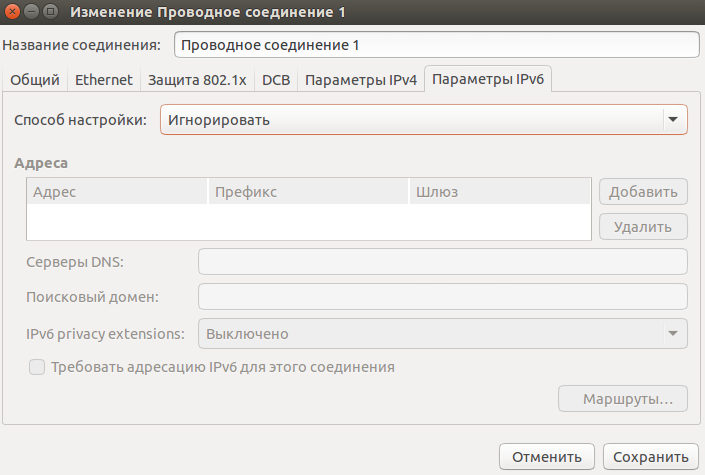
\includegraphics[width=0.6\linewidth]{network_2}}
\caption{ Параметры IPv6 для проводного соединения }
\label{network_2:network_2}
\end{figure}

\begin{figure}[h!]
\center{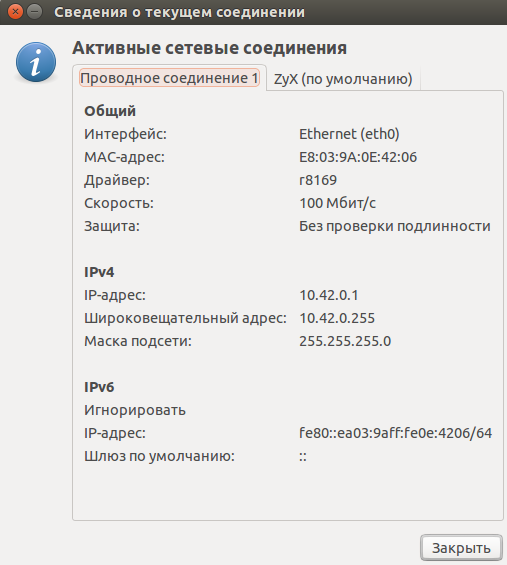
\includegraphics[width=0.6\linewidth]{network_3}}
\caption{ Параметры IPv4 для беспроводного соединения }
\label{network_3:network_3}
\end{figure}

\begin{figure}[h!]
\center{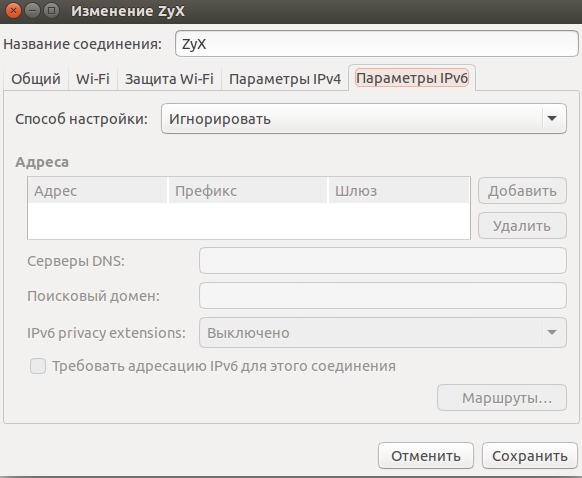
\includegraphics[width=0.6\linewidth]{network_4}}
\caption{ Параметры IPv6 для беспроводного соединения }
\label{network_4:network_4}
\end{figure}

Все остальные настройки оставить по умолчанию.


\begin{figure}[h!]
\center{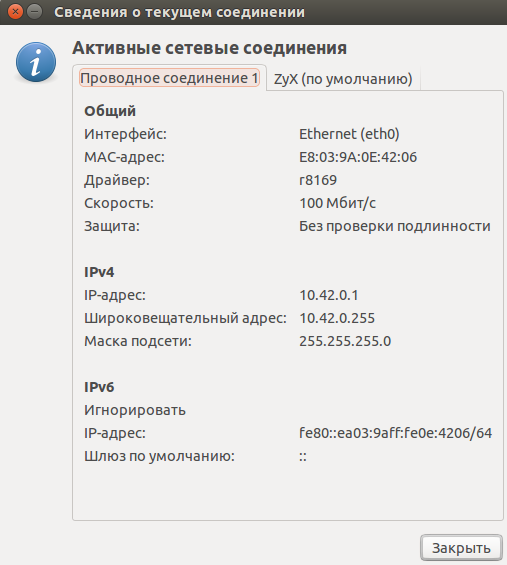
\includegraphics[width=0.6\linewidth]{network_5}}
\caption{ Сведения о проводном соединении }
\label{network_5:network_5}
\end{figure}

\begin{figure}[h!]
\center{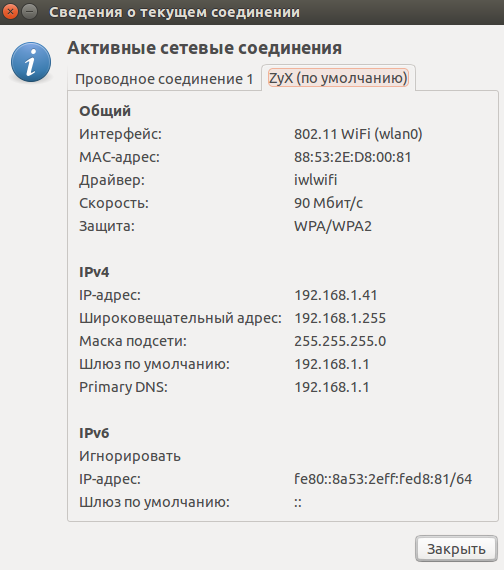
\includegraphics[width=0.6\linewidth]{network_6}}
\caption{ Сведения о беспроводном соединении }
\label{network_6:network_6}
\end{figure}



\clearpage





